\documentclass[14pt]{beamer}
\usetheme{Dresden}
\usecolortheme{orchid}

\usepackage{xcolor}
\usepackage{listings}
\usepackage{courier}
\usepackage{graphicx}
\usepackage{amsmath}
\usepackage{algorithm2e}

\usefonttheme[onlymath]{serif}

\definecolor{mGreen}{rgb}{0,0.6,0}
\definecolor{mGray}{rgb}{0.5,0.5,0.5}
\definecolor{mPurple}{rgb}{0.8,0,0.82}
\definecolor{backgroundColour}{rgb}{0.95,0.95,0.92}

\lstdefinestyle{CStyle}{
    backgroundcolor=\color{backgroundColour},   
    commentstyle=\color{mGreen},
    keywordstyle=\color{magenta},
    numberstyle=\tiny\color{mGray},
    stringstyle=\color{mPurple},
    basicstyle=\ttfamily\footnotesize,
    breakatwhitespace=false,         
    breaklines=true,                 
    captionpos=b,                    
    keepspaces=true,                 
    numbers=left,                    
    numbersep=5pt,                  
    showspaces=false,                
    showstringspaces=false,
    showtabs=false,                  
    tabsize=2,
    language=C
}

\lstset{basicstyle=\footnotesize\ttfamily,breaklines=true}
\lstset{framextopmargin=50pt,frame=bottomline}

\title{ENGG1003 - Tuesday Week 2}
\subtitle{Calculating Pi\\C Arithmetic\\Datatypes}
\author{Brenton Schulz}
\institute{University of Newcastle}
\date{\today}

\begin{document}
\titlepage

\begin{frame}
\frametitle{Case Study: Calulating $\pi$}
\begin{itemize}
\item Computers are \textit{really} good at repetitive things
\item Lets use this fact to calculate $\pi$ using a ``monte-carlo'' method
	\begin{itemize}
		\item Informally, these are methods which solve problems by repeating the same thing with different inputs until patterns emerge
		\item It could repeat millions or billions of times
		\item Name comes from the Monaco Principality's high concentration of casinos
	\end{itemize}
\item Algorithm pseudocode will be written before an implementation in C
\end{itemize}
\end{frame}

\begin{frame}
\frametitle{Case Study: Calulating $\pi$}
Consider a quadrant of a unit circle ($r=1$) with a square around it:
\begin{columns}
\begin{column}{0.5\textwidth}
\begin{itemize}
\small{
\item Area of the square $A_1 = 1$\\
\item Area of the circle quadrant $A_2 =\frac{\pi r^2}{4} = \frac{\pi}{4}$ \\
\item Ratio of areas $\frac{A_2}{A_1} = \frac{\pi}{4}$
\item Therefore $\pi = 4\times \frac{A2}{A1}$
}
\end{itemize}
\end{column}
\begin{column}{0.5\textwidth}
\begin{figure}
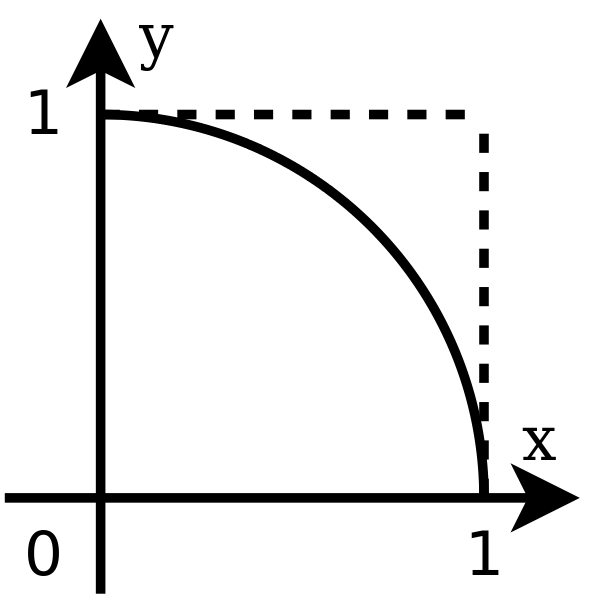
\includegraphics[width=0.9\textwidth]{pi.png}
\end{figure}
\end{column}
\end{columns}
\end{frame}

\begin{frame}
\frametitle{Case Study: Calulating $\pi$}
\begin{columns}
\begin{column}{0.5\textwidth}
\begin{itemize}
\small{
\item We can't calculate the area ratio without knowing $\pi$
\item Estimate it by:
\begin{itemize}
	\item Randomly picking many points inside the square
	\item Test if the point is inside the circle with $x^2 + y^2 < 1$
	\end{itemize}
}
\end{itemize}
\end{column}
\begin{column}{0.5\textwidth}
\begin{figure}
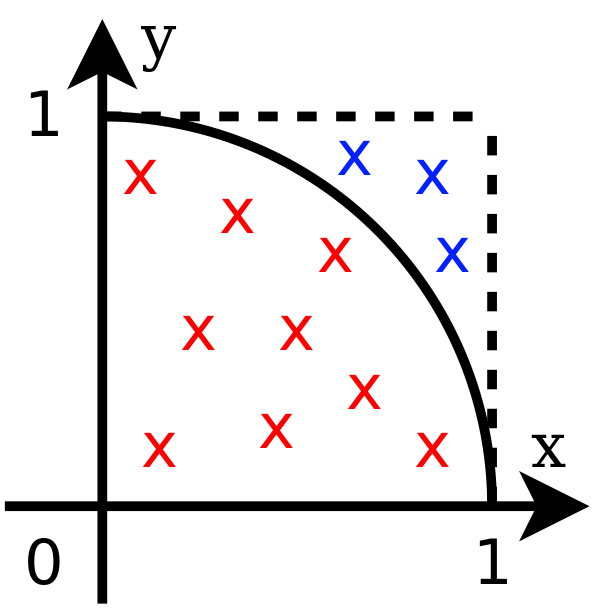
\includegraphics[width=0.9\textwidth]{pi-dots.png}
\end{figure}
\end{column}
\end{columns}
\begin{itemize}
\item $\pi \approx 4 \times \frac{\textrm{Number of points which land inside circle}}{\textrm{Total number of points tested}} = 4 \times \frac{9}{12} = 3$
\end{itemize}
\end{frame}

\begin{frame}
\frametitle{Algorithm for Calculating $\pi$}

\begin{itemize}
\item How can the above \textit{mathematics} be turned into an \textit{algorithm}?
\item The algorithm needs to repeat the \textit{same thing} multiple times
	\begin{itemize}
			\item This implies use of a loop
			\item The loop's \textit{exit condition} needs to be defined
	\end{itemize}
\item As the loop repeats, we need to keep track of the following \textit{variables}:
		\begin{itemize}
			\item The number of points tested
			\item The number of points which landed inside the circle
			\item The $(x,y)$ coordinates of the point under test
		\end{itemize}


\end{itemize}	 
\end{frame}

\begin{frame}
\frametitle{Algorithm for Calculating $\pi$}
\begin{itemize}
\item The number of points tested will be an \textit{integer}, we will call it \texttt{countTotal}
\item The number of points found to be inside the circle is also an integer, we will call it \texttt{countInside}
\item Before these variables are used they should be \textit{initialised}
	\begin{itemize}
		\item ie: The algorithm will explicitly include \texttt{countTotal = 0} and \texttt{countInside = 0}
		\item So-called \textit{uninitialised} variables have undefined (or random) values
	\end{itemize}
\end{itemize}
\end{frame}

\begin{frame}
\frametitle{Algorithm for Calculating $\pi$}
\begin{itemize}
\item Incrementing the \texttt{countInside} variable is \textit{conditional} on the values of $x$ and $y$
	\begin{itemize}
		\item This implies \texttt{IF...ENDIF} \textit{flow control}
	\end{itemize}
\item The condition on incrementing \texttt{countInside} is $x^2 + y^2 < 1$
\item Incrementing a variable in pseudocode takes the form:
	\begin{itemize}
		\item \texttt{variable = variable + 1}
		\item This can be read as ``variable \textit{becomes} variable plus 1''
		\item Mathematics would write: $x_{n+1} = x_n + 1$
	\end{itemize}
\end{itemize}
\end{frame}

\begin{frame}
\begin{itemize}
\item The point under test needs two ``real'' variables: \texttt{x} and \texttt{y}
	\begin{itemize}
 		\item ``Real'' is the generic term for a number with integer and fractional components. Eg: 1.45
	\end{itemize}
\item These values take new random values each loop
\item The pseudocode doesn't need to describe how a random number is generated
	\begin{itemize}
		\item Stating: ``\texttt{x = a random number between 0 and 1}'' is totally acceptable
	\end{itemize}
\item At the end of the algorithm the final step will be $\pi = 4\times \frac{\texttt{countInside}}{\texttt{countTotal}}$
\end{itemize}
\end{frame}


\begin{frame}
\frametitle{Algorithm for Calculating $\pi$}
{\footnotesize
\texttt{BEGIN\\
\quad integer countTotal = 0\\
\quad integer countInside = 0\\
\quad WHILE countTotal < A large number\\
\quad \quad x = random number between 0 and 1\\
\quad \quad y = random number between 0 and 1\\
\quad \quad countTotal = countTotal + 1\\
\quad \quad IF $x^2 + y^2 < 1$\\
\quad \quad \quad countInside = countInside + 1\\
\quad \quad ENDIF\\
\quad ENDWHILE\\
\quad pi = 4*countInside/countTotal\\
\quad PRINT pi\\
END\\
}
}
\end{frame}

\begin{frame}
\frametitle{Missing Knowledge for C Implementation}
\begin{itemize}
\item More information about arithmetic
\begin{itemize}
	\item Relational operators look useful
	\item Is there a neat way to do \texttt{count=count+1}?
	\item \texttt{countInside} and \texttt{countTotal} are both integers. What happens when we divide?
\end{itemize}
\item Datatypes and how they are handled in arithmetic statements
\item How do we generate random numbers?
\item Syntax for WHILE loops and IF statements
\end{itemize}
\end{frame}

\begin{frame}
\frametitle{C Arithmetic}
\begin{itemize}
\item Basic arithmetic was seen in the lab
\begin{itemize}
\item You all did the lab, right?
\end{itemize}
\begin{table}[H]
\centering
\begin{tabular}{|l|c|}
\hline
Operation      & C Symbol \\
\hline
Addition       & +        \\
Subtraction    & -        \\
Multiplication & *        \\
Division       & /       \\
\hline
\end{tabular}
\caption{Basic arithmetic operators in C}
\end{table}
\item Complex expressions can be built from these operators and parentheses
\end{itemize}
\end{frame}

\begin{frame}
\frametitle{C Arithmetic}
Examples:
\begin{small}
\begin{table}
\centering
\begin{tabular}{cc}
\vspace{2mm}
$z = x^2 + 5(y + b)$ & \texttt{z = x*x + 5*(y + b);} \\
\vspace{2mm}
$u = \frac{x + 1}{x - 1}$ & \texttt{u = (x + 1)/(x - 1);} \\
$v = z^3 + \frac{5(y + b)}{2}$ & \texttt{v = z*z*z+(5*(y + b))/2;} \\
\end{tabular}
\end{table}
\end{small}

\begin{itemize}
\item Multiplication is not assumed. If you write \texttt{5(y+b)} the compiler will generate a syntax error.
\item To be valid C expressions the semicolon is required.
\end{itemize}
\end{frame}

\begin{frame}
\frametitle{C Arithmetic}
\begin{itemize}
\item C supports two time-saving \textit{unary} operators:
\begin{itemize}
\item Very useful in loops.
\end{itemize}

\begin{table}
\centering
\begin{tabular}{|c|c|c|}
\hline
Operation & C Syntax & Replaces\\
\hline
Increment & \texttt{x++;} or \texttt{++x;} & \texttt{x = x + 1;} \\
Decrement & \texttt{x--;} or \texttt{--x;} & \texttt{x = x - 1;} \\
\hline
\end{tabular}
\end{table}

\item It also supports the following shorthand syntax:

\begin{table}
\centering
\begin{tabular}{|c|c|c|}
\hline
\texttt{x = x + y;} & \texttt{x += y;} \\
\texttt{x = x - y;} & \texttt{x -= y;} \\
\texttt{x = x * y;} & \texttt{x *= y;} \\
\texttt{x = x / y;} & \texttt{x /= y;} \\
\hline
\end{tabular}
\end{table}
\end{itemize}
\end{frame}

\begin{frame}
\frametitle{C Arithmetic}
What's the difference between \texttt{x++} and \texttt{++x}?
\begin{itemize}
\item \texttt{x++} is a \textit{post-increment}
\item \texttt{++x} is a \textit{pre-increment}
\item If they appear in an arithmetic expression, pre-increment is processed \textit{before} the variable is used and post-increment is processed \textit{after} it is used.
\item In isolation there is no difference.
\end{itemize}
\end{frame}

\begin{frame}[fragile]
\frametitle{Increment Example}
\begin{lstlisting}[style=CStyle]
#include <stdio.h>
int main() {
	int x = 0;
	int y = 0;
	int z = 0;
	y = ++x + 10;
	printf("Pre-increment: %d\n", y);
	y = z++ + 10;
	printf("Post-increment: %d\n", y);
	return 0;
}
\end{lstlisting}
Pre/post-inc/decrements have many applications, more details in coming weeks.
\end{frame}

\begin{frame}
\frametitle{Modulus}
\begin{itemize}
\item Computers frequently only deal with integers
\item Integer division in C ignores (truncates) any fractional component
\item The \textit{modulus} operator provides the remainder after division
\begin{itemize}
	\item Implemented with the \texttt{\%} character
	\item \texttt{a \% b =} remainder of \texttt{a / b}
	\item Very useful for tasks performed every \textit{nth} loop
\end{itemize}
\item Example:
	\begin{itemize}	
		\item \texttt{10 / 3 = 3}
		\item \texttt{10 \% 3 = 1}
	\end{itemize}
\end{itemize}
\end{frame}

\begin{frame}[fragile]
\frametitle{Modulus Example - Factor Testing}
\begin{lstlisting}[style=CStyle]
#include <stdio.h>
int main() {
	int x;
	int y;
	printf("Enter an integer: ");
	scanf("%d", &x);
	printf("Enter another integer: ");
	scanf("%d", &y);
	if(x % y == 0) { // ie: if the remainder is zero
		printf("%d is a factor of %d\n", y, x);
	} else {
		printf("%d is NOT a factor of %d\n", y, x);
	}
	return 0;
}
\end{lstlisting}
\end{frame}

\begin{frame}
\frametitle{Relational Operators}
\begin{itemize}
\item C supports six \textit{relational} operators:
\begin{table}[H]
\centering
\begin{tabular}{|l|c|}
\hline
Operation      & C Symbol \\
\hline
Less than       & $\texttt{<}$        \\
Less than or equal to    & $\texttt{<=}$\\
Greater than & $\texttt{>}$        \\
Greater than or equal to       & $\texttt{>=}$       \\
Equal to & \texttt{==} \\
Not equal to & \texttt{!=} \\
\hline
\end{tabular}
\caption{Relational operators in C}
\end{table}
\end{itemize}
\end{frame}

\begin{frame}
\frametitle{Relational Operators}
\begin{itemize}
\item The result of a relational operation is \texttt{0} or \texttt{1}
	\begin{itemize}
		\item C treats \texttt{0} as Boolean FALSE and non-zero as TRUE
	\end{itemize}
\item They are typically used as flow control conditions
	\begin{itemize}
		\item \texttt{if(\textit{condition}) \{\textit{statements}\}}
		\item \texttt{while(\textit{condition}) \{\textit{statements}\}}
	\end{itemize}
\item While we're here: the above is the correct syntax for IF and WHILE flow control in C
\end{itemize}
\end{frame}

\begin{frame}[fragile]
\frametitle{Modulus Example 1 - Printing Every \textit{nth} Loop}
\begin{lstlisting}[style=CStyle]
#include <stdio.h>
int main() {
	int x = 0;
	while(x < 1000)
	{
		// Presumably something useful is done with x
		// inside this loop
		if(x%100 == 0)
			printf("%d\n", x);
	}
	return 0;
}
\end{lstlisting}
\end{frame}

\begin{frame}[fragile]
\frametitle{Modulus Example 2 - Finding Factors}

\begin{lstlisting}[style=CStyle,basicstyle=\ttfamily\scriptsize]
#include <stdio.h>
int main() {
	int input;
	int x;
	printf("Enter an integer to factorise: ");
	scanf("%d", &input);
	x = input;
	while(x > 0) {
		if(input % x == 0) // ie: if the remainder is zero
			printf("%d is a factor of %d\n", x, input);
		x--;
	}
	return 0;
}
\end{lstlisting}
{\small
Observe that the \texttt{while()} loop loops over every value of \texttt{x} from \texttt{input} to \texttt{1}. We will discuss a flow control method designed for this (the \texttt{for} loop) later.
}
\end{frame}

\begin{frame}
\frametitle{C Arithmetic Operator Precedence}
\begin{itemize}
\item C has an ``order of operations''
\item eg: \texttt{1+5*2} evaluates to \texttt{11}
\item Multiplication and division first
\item Addition and subtraction second
\item Relational operators somewhere below that
\item If in doubt: force order with parentheses
	\begin{itemize}
		\item This makes the code more readable
		\item It doesn't cost you anything
		\item C compilers understand algebra and will optimise inefficient expressions automatically
	\end{itemize}

\end{itemize}
\end{frame}

\begin{frame}
\frametitle{Data Types}
\begin{itemize}
\item In C, all variables are \textit{declared} before use
\item Declaration specifies the variable's:
	\begin{itemize}
		\item Datatype
		\item Name
		\item An \textit{initialisation value} (optional)
			\begin{itemize}
				\item Always assume uninitialised variables have random values! Behaviour varies between compilers and target platforms.
			\end{itemize}
	\end{itemize}
\item C is a ``strongly-typed'' language
	\begin{itemize}
		\item Every variable has a fixed type
	\end{itemize}
\end{itemize}
\end{frame}

\begin{frame}
\frametitle{Integer Data Types}
\begin{itemize}
\item There are several integer data types
\item They vary by their:
	\begin{itemize}
		\item Size
		\item Support for negative numbers
	\end{itemize}
\item C integer types can be 1, 2, 4, or 8 bytes long
	\begin{itemize}
		\item The sizes vary by platform
	\end{itemize}
\item Each type can be \textit{signed} or \textit{unsigned}
	\begin{itemize}
		\item Unsigned number are never negative but you get double the value range
	\end{itemize}
\end{itemize}
\end{frame}

\begin{frame}
\frametitle{Integer Data Types}
\begin{itemize}
\item C includes the \texttt{sizeof()} expression so that a program can discover the size of a data type
\item The size (given in bytes) defines the \textit{value range}
\item On a modern 64-bit Linux desktop machine:
\end{itemize}
\begin{table}[]
\begin{tabular}{llll}
Type & Bytes & Bits & Value Range                               \\
char      & 1            & 8           & -128, +127                                \\
short     & 2            & 16          & -65536, 65535                             \\
int       & 4            & 32          & -2147483648, 2147483647                   \\
long      & 8            & 64          & -9223372036854775808, ...
\end{tabular}
\end{table}
\end{frame}

\begin{frame}
\frametitle{Unsigned Integers}
\begin{itemize}
\item Unsigned integers are \textit{always positive}
\item They are the same size as their signed counterparts
\item eg: \texttt{unsigned char} is 1 byte and has a value range of \texttt{0} to \texttt{255}
\end{itemize}
\end{frame}

\begin{frame}
\frametitle{Why Care About Data Types?}
\begin{itemize}
\item You may be thinking ``why not make everything a \texttt{long}?''
\item Answer: speed and memory
\item Smaller types use less RAM
\item Arithmetic on a type larger than the target platform's \textit{native size} is slow
\item Matters if you store millions of the same type
\item Makes a \textit{huge} difference on embedded targets
\begin{itemize}
	\item Don't declare 32-bit variables on an 8-bit AVR microcontroller \textit{unless you have to}
\end{itemize}
\end{itemize}
\end{frame}

\begin{frame}[fragile]
\frametitle{Integer Division Example}
What is the output of each \texttt{printf()} statement?
\begin{lstlisting}[style=CStyle]
#include <stdio.h>
int main() {
	printf("%d\n", 9/10);
	printf("%f\n", 9/10);
	printf("%f\n", 9.0/10);
	printf("%f\n", 9/10.0);
	printf("%f\n", (float)9/10);
	return 0;
}
\end{lstlisting}
\end{frame}

\begin{frame}
TODO: Keep hacking until we've implemented $\pi$.
\end{frame}

\end{document}
